\section{Experiments}
\label{sec:eval}

In this section, we evaluate our system with two tasks: link prediction
and triple classification.
Then we show examples of detail schemas inferred by our system, and analyze the result.

\subsection{Experimental Setup}

\textbf{Knowledge bases.} 
We use three knowledge bases throughout our experiments: 
FB15k, FB15k-type and FB (full version).
As the main benchmark dataset, FB15k \cite{bordes2013translating}
is a subset of Freebase containing 14951 entities and 1345 predicates.
\KZ{Rephrase this, not clear what you mean: Triples in FB15k are 
split into training / validation / test parts,
since all evaluating triple facts come from OpenIE system, 
we only use triples from training split, keeping a fair comparison with 
state-of-the-art approaches.}
Note that FB15k doesn't contain IsA relationship, thus we construct 
a new knowledge base called FB15k-type by adding type information 
of all entities into FB15k.
Besides, we use Freebase dump as of June 2015~\cite{freebase:datadumps} 
as the full version of FB.
We use \KZ{these two complementary knowledge bases} in link prediction task.
\tabref{tab:fb-size} shows the statistics of these KBs.

\noindent
\textbf{OpenIE datasets.}
We select PATTY \cite{nakashole2012patty} as the OpenIE dataset.
PATTY contains more than 200,000 different relation synsets
with millions of entity pairs extracted from Wikipedia.
Each entity in PATTY is linked to Freebase through a unique Wikipedia page.
From top 1,000 distinct PATTY relations sorted by the number of 
relation instances, we randomly pick 100 relations for evaluation.
Each relation contains 180 instances on average, and we split them into
training / validation / test sets (64\% : 16\% : 20\%).
By manual inspecting, 18 relations are considered complex relations, 
and while the remaining relations are classified as ``ordinary'' relations.

\begin{table}[ht]
	\small
	\centering
	\caption{Statistics of Freebase used in experiments. \KQ{to be updated.}}
	\begin{tabular}{|c|c|c|c|}
		%\toprule
		\hline
		Dataset				&	FB15k	&	FB15k-type	&	 FB		\\
        \hline
		%Ordinary entities	& 50,718,028	& 3,000,000		&		\\
        %\hline
        %Mediator entities	& 36,131,437	& 7,301,261		&		\\
		%\hline
		Total entities		&	14,951	&	14,951	&	86,849,465	 \\
		\hline
		Distinct relations	&	1,345	&	1,345	&	4,932	\\
        \hline
		Types 				&	0		&	xxxx	&	2,071	\\
		\hline
		IsA relationships	&	0		&	yyyy	&	zzzz	\\
		\hline
		Triple facts		&	483,142	&	483,142	& 280,788,583	\\
		\hline
	\end{tabular}%
	\label{tab:fb-size}%
\end{table}


\noindent
\textbf{State-of-the-art comparisons.}
For embedding techniques, we take TransE \cite{bordes2013translating},
KALE \cite{guo2016jointly}, TEKE \cite{wang2016text} and 
HOLE \cite{} as our comparisons.
TransE models the confidence of a triple fact as vector translations on the
embeddings of the predicate and two entity arguments.
%TransE models a relationship as operating translations on the embeddings of
%subject and object entities. \KQ{Change all subject, object into head, tail??}
KALE and TEKE are two extensions of TransE.
KALE introduces logical rules as the combination of atom triple facts with logical connectives,
therefore the model can learn embeddings from both positive triples and rules.
TEKE enables each relation to own different representations for different subject and object
entities, by leveraging the rich context information of a triple fact in web text corpus.
HOLE is a novel compositional embedding model for representing relationships,
which is based on the circular correlation of entity vectors.

For rule induction techniques, we compare with two models:
SFE \cite{gardner2015efficient} and AMIE+ \cite{}.
One traditional model, called Path Ranking Algorithm \cite{lao2011random},
extracts all possible paths connecting subject and object entities,
then learns a feature-based model to represent each relation,
and SFE is an extension of PRA model, by adding extra subgraph features 
from the surrounding of subject and objects entities in the knowledge base.
AMIE+ first searches possible structures, and then calculates the confidence score 
of each structure by a simple counting strategy in positive triple facts
(without the step of weight learning).
We also considered Coupled PRA model \cite{} as a comparison. However, 
because different relations share almost no entity
pairs in the OpenIE dataset,
the model would degenerate into the traditional PRA model
and hence stricted superseded by SFE.

\noindent
\textbf{Implementation detail.}
We evaluate our approach under several settings.
In candidate generation step, we compare two settings: 
``use-skeleton-only'' and ``use-whole-schema'', based on 
whether to explore constraints.
The first specification only extract path candidates without generating 
constraints, while the latter one is free to use all candidate schemas.
In schema inference step, we compare two strategies ``random walk'' 
and ``zero-one'', described in \secref{sec:schema}. 
\KQ{Will update approach part, mentioning these notations.}
For each specification, we select the size of priority queue in 
\{1000, 2000, 3000, 4000, 5000\},
in order to observe how the result varies with the number of candidate schemas.
We set the maximum length of a skeleton $\tau = 3$,
tune the minimum support $\gamma$ as in \{5\%, 10\%, 15\%, 20\%\},
and the smoothing parameter $\alpha$ in \{0, 1e-6, 1e-5, 1e-4\}.
\KZ{Shall we also eval the effect of different $\tau$? To justify
why 3 is the right choice.}
%TODO: Add detail about the other state-of-the-arts.

\subsection{Link Prediction}
This task is to predict the missing object in the triple ($e_1$, $r$, $?$),
or the missing subject in ($?$, $r$, $e_2$).
Following the evaluation protocol of KALE \cite{guo2016jointly},
for each triple ($e_1$, $r$, $e_2$) in testing set, 
we replace the subject entity $e_1$
by any other corrupted entities $e'_1$ in the knowledge base, \KZ{What do you mean corrupted?}
then calculate the score of each ($e'_1$, $r$, $e_2$) triple and rank them in descending order,
returning the rank of the correct subject entity $e_1$.
Similarly, we can get the rank of $e_2$ at object side.
To be consistent with state-of-the-art systems, we aggregate over all testing triples
and report three evaluation metrics: 
the mean reciprocal rank (MRR), the median value
of the ranks (MED), and the proportion of ranks no larger than $n$ (Hit@$n$).
\KZ{What about macro F1?}

Due to the existence of many-to-one relations, some corrupted triples ($e'_1$, $r$, $e_2$)
are actually correct and already observed in the dataset.
In this case, we follow TransE \cite{bordes2013translating}
and create two settings called ``raw'' and ``filtered''.
In the filtered setting, we remove such \KZ{corrupted triples} from the triple list
before calculating the rank of each prediction.
Conversely, in the raw setting, we don't remove any corrupted triples.

We first evaluate our approach between different settings.
Combining different strategies in candidate generation step and 
schema inference step, we have 4 experimental settings in total.
For each setting, we tune parameters $\gamma$ and $\alpha$, such that
the model reaches the best MRR score (filtered setting) on the validation set.
We perform the evaluation on FB15k under filtered setting \KZ{What is this
setting? Never mentioned before?}.
\figref{fig:trend-with-budget} shows how the MRR results 
\KQ{on validation set}, vary with the number of candidate schemas.
From the results, we observe that:
1) The MRR result increases with the number of candidate schemas in 
every setting, which indicates that larger number of candidates 
leads to a better model.
2) Compare with strategies on candidate generation, use-whole-schema 
outperforms use-skeleton-only, demonstrating the capability of constraints
to represent natural language relations.
3) \KQ{random walk v.s. zero-one, need to get real results before the analysis.}

%\KQ{Figure to be plotted: budget 1k~5k  *  4 different specifications.}
\begin{figure}[th]
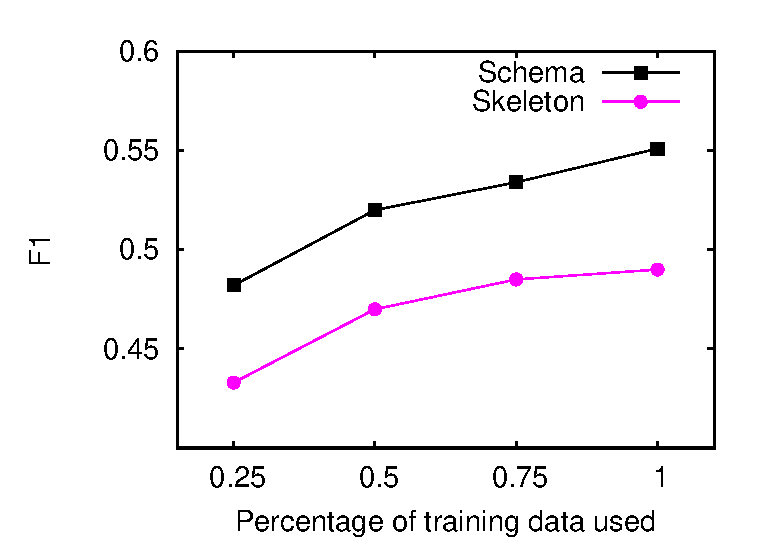
\epsfig{file=trend.eps, width=0.65\columnwidth}
\centering
\caption{
	The trend of link prediction results on FB15k (filtered setting).
	X axis: size of priority queue,
	Y axis: MRR score. \KQ{content to be updated.}
}
\label{fig:trend-with-budget}
\end{figure}

Then we compare our approach with state-of-the-art models.
\KQ{Need to say a little bit about the parameters we used here.}
\tabref{tab:link-pred-raw} and \tabref{tab:link-pred-filtered} 
show the results in
the raw setting and filtered setting respectively.
\KZ{Due to memory issues of the code, SFE method failed to produce any result.
This is a bit strange: you pick SFE as a comparison but it doesn't work for
link prediction at all! Better fix this!}
As we can see, our approach outperforms both embedding and 
other rule induction models.
Comparing the results on different set of relations,
the improvements on complex relations are much more significant than those
on ordinary relations, indicating the usefulness of the extra constraints 
in representing complex relations.
Besides, the link prediction results on natural language relations 
are relatively lower than
those results evaluated on FB15k relations \cite{guo2016jointly}.
Two possible reasons are: 1) triples collected from OpenIE system may 
contain more noise than carefully curated knowledge bases; 
2) in our dataset, each relation has fewer training instances 
(115 triples per relation on average), while in the experiments
of Guo et al. \shortcite{guo2016jointly}, that number is 360.

\KQ{Coming soon: compare on FB15k-type and FB-full.}


\begin{table*}[ht]
	\small
	\centering
	\caption{Link prediction results on FB15k (raw setting).}
	\begin{tabular}{|c|ccccc|ccccc|ccccc|}
		%\toprule
		\hline
				&	\multicolumn{5}{c|}{Complex relations}
				&	\multicolumn{5}{c|}{Ordinary relations}
				&	\multicolumn{5}{c|}{Overall}	\\
		\cline{2-16}	
		\multirow{2}{*}{}	&	\multirow{2}{*}{MRR}	&	\multirow{2}{*}{MED}	&	\multicolumn{3}{c|}{Hit@n(\%)}
							&	\multirow{2}{*}{MRR}	&	\multirow{2}{*}{MED}	&	\multicolumn{3}{c|}{Hit@n(\%)}
							&	\multirow{2}{*}{MRR}	&	\multirow{2}{*}{MED}	&	\multicolumn{3}{c|}{Hit@n(\%)}	\\
				&	&	&	3	&	5	&	10	
				&	&	&	3	&	5	&	10	
				&	&	&	3	&	5	&	10	\\
		\hline
		TransE
				&	0.089	&	75.0	&	11.7	&	17.2	&	23.2
				&	0.081	&	66.0	&	 8.1	&	12.1	&	19.6
				&	0.082	&	68.0	&	 8.9	&	13.2	&	20.4	\\
		KALE	
				&	0.142	&	47.0	&	17.5	&	23.4	&	30.5
				&	0.104	&	42.0	&	11.2	&	16.0	&	24.0
				&	0.112	&	\textbf{43.0}	&	12.5	&	17.6	&	25.4	\\
		TEKE	
				&	0.xxx	&	0.yyy	&	zz.z	&	zz.z	&	zz.z
				&	0.xxx	&	0.yyy	&	zz.z	&	zz.z	&	zz.z
				&	0.101	&	974.0	&	10.9	&	15.7	&	24.1	\\
		HOLE
				&	0.153	&	55.0	&	16.0	&	20.5	&	27.4
				&	0.097	&	51.0	&	 9.1	&	13.9	&	22.2
				&	0.109	&	52.0	&	10.5	&	15.4	&	23.3	\\
		%\hline
		%SFE-AnyRel
		%SFE-OneSide
		AMIE+
				&	0.164	&	76.3	&	18.2	&	21.9	&	26.6
				&	0.107	&	68.3	&	11.3	&	15.8	&	22.6
				&	0.119	&	69.5	&	12.7	&	17.1	&	23.5	\\
		Ours
				&	0.225	&	42.5	&	24.3	&	27.8	&	34.7
				&	0.158	&	43.0	&	16.9	&	21.0	&	28.5
				&	\textbf{0.172}	&	\textbf{43.0}	&	\textbf{18.5}	&	\textbf{22.5}	&	\textbf{29.8}	\\
		\hline
	\end{tabular}
	\label{tab:link-pred-raw}
\end{table*}


\begin{table*}[ht]
	\small
	\centering
	\caption{Link prediction results on FB15k (filtered setting).}
	\begin{tabular}{|c|ccccc|ccccc|ccccc|}
		%\toprule
		\hline
				&	\multicolumn{5}{c|}{Complex relations}
				&	\multicolumn{5}{c|}{Ordinary relations}
				&	\multicolumn{5}{c|}{Overall}	\\
		\cline{2-16}	
		\multirow{2}{*}{}	&	\multirow{2}{*}{MRR}	&	\multirow{2}{*}{MED}	&	\multicolumn{3}{c|}{Hit@n(\%)}
							&	\multirow{2}{*}{MRR}	&	\multirow{2}{*}{MED}	&	\multicolumn{3}{c|}{Hit@n(\%)}
							&	\multirow{2}{*}{MRR}	&	\multirow{2}{*}{MED}	&	\multicolumn{3}{c|}{Hit@n(\%)}	\\
				&	&	&	3	&	5	&	10	
				&	&	&	3	&	5	&	10	
				&	&	&	3	&	5	&	10	\\
		\hline
		TransE
				&	0.097	&	69.0	&	13.0	&	18.7	&	25.0
				&	0.092	&	62.0	&	 9.7	&	14.2	&	22.2
				&	0.094	&	63.0	&	10.4	&	15.2	&	22.8	\\
		KALE	
				&	0.153	&	43.0	&	19.9	&	25.5	&	32.5
				&	0.118	&	39.0	&	12.9	&	18.0	&	26.1
				&	0.125	&	\textbf{39.0}	&	14.4	&	19.6	&	27.5	\\
		TEKE	
				&	0.xxx	&	0.yyy	&	zz.z	&	zz.z	&	zz.z
				&	0.xxx	&	0.yyy	&	zz.z	&	zz.z	&	zz.z
				&	0.114	&	973.0	&	12.6	&	17.9	&	26.3	\\
		HOLE
				&	0.162	&	50.5	&	17.4	&	21.8	&	29.0
				&	0.109	&	47.0	&	10.9	&	16.1	&	24.9
				&	0.121	&	47.0	&	12.3	&	17.3	&	25.8	\\
		%\hline
		%SFE-AnyRel
		%SFE-OneSide
		AMIE+
				&	0.180	&	73.8	&	18.6	&	22.4	&	27.5
				&	0.120	&	63.5	&	12.5	&	17.0	&	23.6
				&	0.132	&	65.0	&	13.8	&	18.2	&	24.4	\\
		Ours
				&	0.237	&	41.0	&	25.2	&	29.1	&	35.5
				&	0.171	&	40.0	&	18.4	&	22.4	&	30.5
				&	\textbf{0.185}	&	40.0	&	\textbf{19.9}	&	\textbf{23.8}	&	\textbf{31.5}	\\
		\hline
	\end{tabular}
	\label{tab:link-pred-filtered}
\end{table*}






\subsection{Triple Classification}
This task is to predict whether a new triple ($e_1$, $r$, $e_2$) is correct or not.
As a binary classification task, we need to generate negative triples for evaluations.
Following the strategy used in KALE \cite{guo2016jointly},
for each positive triple in the validation and test set,
we generate 10 negative triples by randomly corrupting the entities, 5 at the subject
position and 5 at the object position. We ensure that each corrupted entity 
has appeared in some other positive triples at the same position,
and all corrupted triples do not exist in either the training, validation or test set.
Then for each relation, we rank all triples (both positive and negative)
by their scores in descending order, and calculate the average precision (AP) for the relation.
As the metric, we report the mean average precision (MAP) aggregated over all relations.

We perform the experiment on FB15k, and \tabref{tab:triple-clsf} shows the result on
different categories of relations.
%Currently: Vrw, schema
Our model outperforms other works, showing us the importance of constraints in a schema.
Observing results of each model, it's interesting to find that all rule induction models
performs much better than embedding techniques, which reveals us that
explicit semantic feature mining could help to find more precise representations,
especially when the training data is small.

\begin{table}[ht]
	\small
	\centering
	\caption{Triple classification results (MAP) on FB15k}
	\begin{tabular}{|c|ccc|}
		%\toprule
		\hline
							& Complex	& Ordinary & Overall 	\\
        \hline
		TransE				&	0.xxx	&	0.yyy	&	0.272	\\
		KALE				&	0.469	&	0.273	&	0.309	\\
		TEKE				&	0.xxx	&	0.yyy	&	0.282	\\
		HOLE				&	0.xxx	&	0.yyy	&	0.308	\\
		\hline
		SFE-Anyrel			&	0.xxx	&	0.yyy	&	\~0.340	\\
		SFE-Onesided		&	0.xxx	&	0.yyy	&	0.zzz	\\
		AMIE+				&	0.499	&	0.337	&	0.367	\\
		Ours				&	0.xxx	&	0.yyy	&	\textbf{0.394}	\\
		\hline
	\end{tabular}
	\label{tab:triple-clsf}
\end{table}



\subsection{Result Analysis}
Finally, we analyze the performance of our learned schemas in more detail.

\begin{figure*}[th]
 \epsfig{file=case_crop.eps, width=1.05\columnwidth, angle=270}
\centering
\caption{An example fragment of schema paraphrasing results.
We list top-3 schemas along with probabilities for each relation.
Circle node indicates entities or variables, the two black circles represents
$x_{subj}$ and $x_{obj}$ respectively. Square node represents a type, and
round square node represents a mediator (auxiliary node to organize an n-ary fact).}
\label{fig:relation-example}
\end{figure*}

\figref{fig:relation-example} shows the paraphrasing results of 
selected relations.
%Show a case-by-case P/R/F1/RR?
The results of top-ranked schemas show us that our paraphrasing system
is able to produce concrete and precise structural representations.
However, in several cases, the system failed to paraphrase the relation into
correct semantics. We have analyzed relations in the above experiments and
find several main causes of error.

1. Relation instances extracted by Open IE system could be incorrect.
PATTY extracts relation instances by mining the dependency path in a sentence,
which may lead to wrong arguments.
For example, given the relation \textit{``served as''}, PATTY extracted
an incorrect entity pair (William Dennison Jr., Ohio) from the sentence
\textit{``Dennison served as the 24th Governor of Ohio and as U.S. Postmaster General ...''},
while the correct object should be ``Governor of Ohio''.

2. PATTY relation synset mixed semantic different but lexical similar
relation patterns, bringing noisy entity pairs in the relation.
For example, in PATTY's \textit{``'s wife''} relation synset, we found a small list of instances
where the object is actually husband.
These instances are due to another pattern in the synset,
\textit{``the wife of''}, which gives the exact opposite semantics.
Though our system is able to filter out noisy instances, the learned schema
distribution would be affected if the percentage of noisy data is large.

3. Knowledge base lacks necessary information for paraphrasing certain relations.
As mentioned before, Freebase doesn't hold knowledge about trivial relations.
Even for non-trivial relations, required predicates could be missing in Freebase.
Given the relation \textit{``(singer) performed in (LOC)''}, FB contains			% synset 0246
neither \textit{place\_visited} nor \textit{hold\_concerts\_in} predicate, therefore
our system is not able to summarize into a precise representation.

4. Sometimes a meaningful schema is filtered out due to the 
the search space limits in candidate searching step.
In relation \textit{``(actor) starring with (actor)''}, 
the length of the most suitable skeleton
\footnote{The skeleton is $actor \rightarrow med. \rightarrow film \rightarrow med. \rightarrow actor$.}
is 4, hence the system failed to discover it under restriction $\tau$ = 3.
\KZ{This is why I said we should evaluate the impact of $\tau$.}

\KZ{After reading this paper, one thing that puzzles me is that why is this
method called paraphrasing natural language relations to knowledge base? The 
approach you are proposing can be used for ordinary KB completion task, right?
In other words we are not making use of the natural language feature at all.
I think perhaps we can include some experiments you did with NL features to
show that NL features are not necessary and explain why. This will clear the
doubt of some readers.}
